%! Author = yessense
%! Date = 04.02.2022

\documentclass{article}
\usepackage[utf8]{inputenc}
\usepackage{graphicx}
\usepackage{hyperref}
\title{dSprites VSA}
\author{ }
\date{ }

\begin{document}

    \maketitle


    \section{Introduction}

    The goal of this work is to extract the features of the image
    and represent them as multidimensional vectors, which, when
    summed up, will allow you to reconstruct the original image.
    Having started with a single object in the scene, we will try
    to move to a set of several objects.


    \section{Datasets}
    The task consists of three consecutive steps for each of
    which a different dataset was created. These datasets are based on
    the dSprites dataset \autoref{fig:dsprites}.
    dSprites is a dataset of 2D shapes procedurally generated
    from 6 ground truth independent latent factors \autoref{tab:features}


    \begin{figure}[ht]
        \centering
        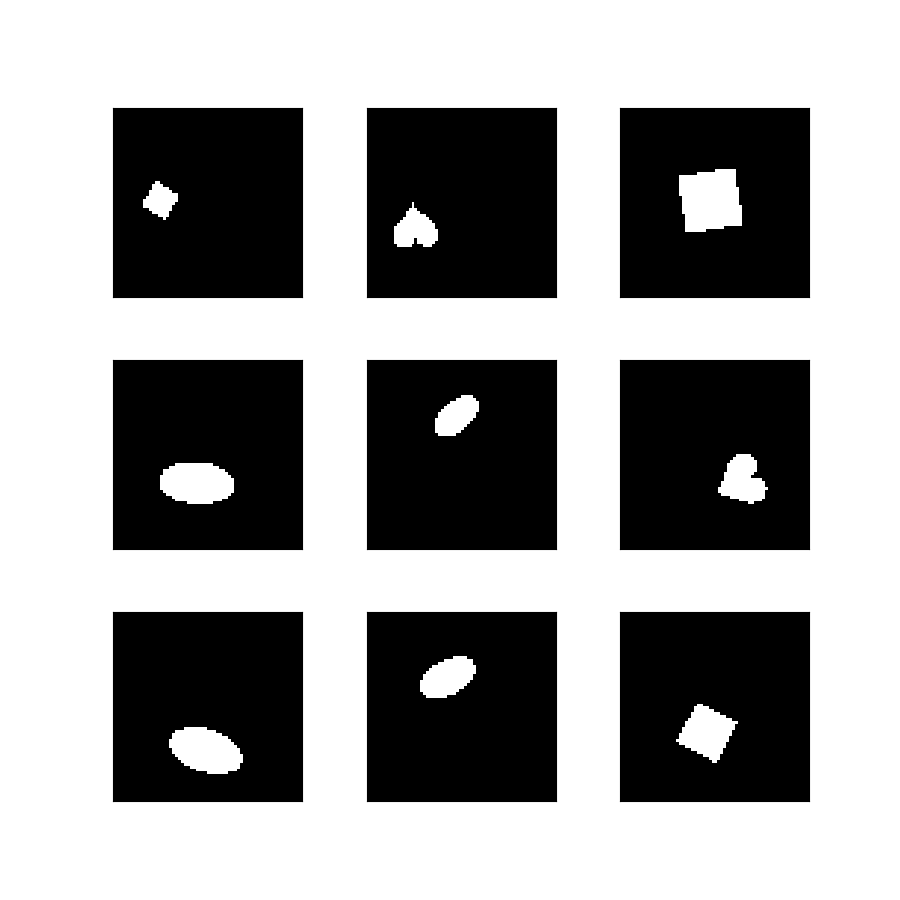
\includegraphics[width=0.3\textwidth]{img/datasets/dsprites}
        \caption{Example of images from dSprites dataset}
        \label{fig:dsprites}
    \end{figure}

    \begin{table}[ht]
        \centering
        \caption{List of features}
        \label{tab:features}
        \begin{tabular}[t]{ll}
            \hline
            Feature     & Distribution                         \\
            \hline
            Shape       & square, ellipse, heart               \\
            Scale       & 6 values linearly spaced in [0.5, 1] \\
            Orientation & 40 values in [0, 2 pi]               \\
            Position X  & 32 values in [0, 1]                  \\
            Position Y  & 32 values in [0, 1]                  \\
            \hline
        \end{tabular}
    \end{table}

    \subsection{Paired dSprites}
    The purpose of creating this dataset is to make it possible to easily
    obtain paired images that differ in a single feature. This is possible
    due to the fact that in the original dataset the images are arranged in
    an orderly manner.
    An example of pairwise images in a dataset can be seen in the
    \autoref{fig:paired_dsprites}
    \begin{figure}[ht]
        \centering
        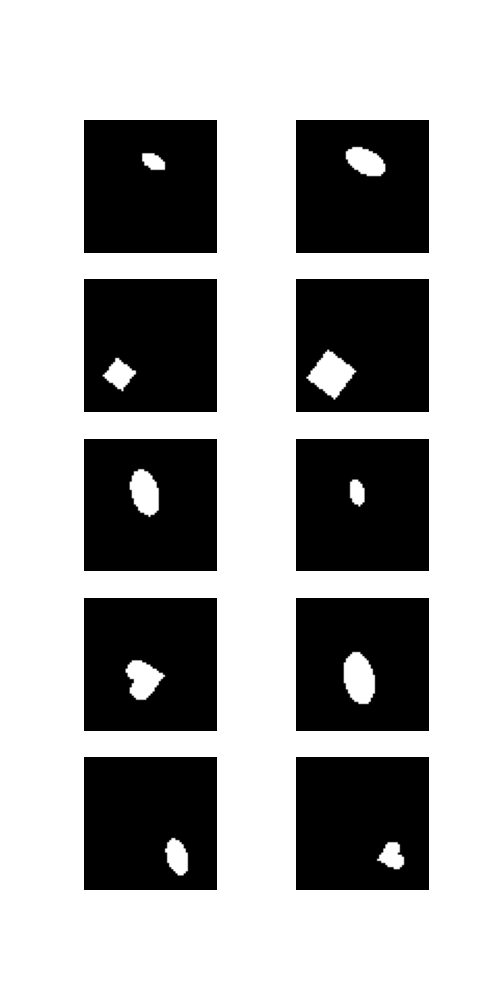
\includegraphics[width=0.3\textwidth]{img/datasets/paired_dsprites}
        \caption{Visualizing Paired dSprites dataset elements}
        \label{fig:paired_dsprites}
    \end{figure}

    \subsection{Scene-dsprites dataset}
    This dataset was created to test the model's ability to reconstruct
    a scene from the sum of object vectors.
    Dataset consists of 2 to 5 non-overlapping figures from dSprites dataset.
    An example of such images on \autoref{fig:scene_dsprites}. This version differs from
    the original multi-dsprites dataset in that the figures do not overlap
    and have the same color.

    \begin{figure}[ht]
        \centering
        
\includegraphics[width=0.7\textwidth]{img/datasets/scene-dsprites}
        \caption{Example of collected scenes in the scene-dsprites dataset}
        \label{fig:scene_dsprites}
    \end{figure}

    \subsection{Paired-Scene-dSprites dataset}
    This dataset combines the capabilities of the first and second dataset.
    There are two objects in the scene image.
    One of these objects can change one feature. \autoref{fig:paired_scene_dsprites}

    \begin{figure}[ht]
        \centering
        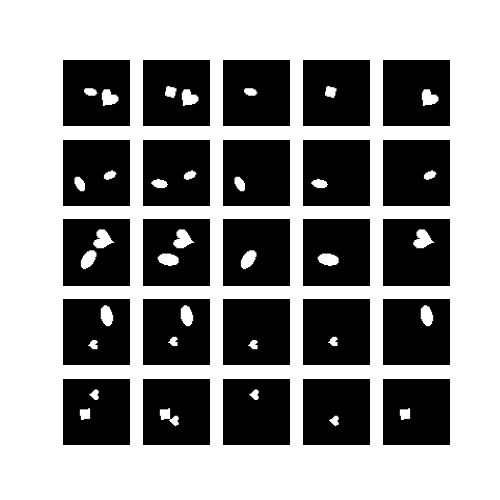
\includegraphics[width=0.6\textwidth]{img/datasets/paired-scenes-dsprites}
        \caption{Example of images from paired-scene-dsprites dataset. From left to right,
            first scene, pair scene, the object to be changed, his pair, second object}
        \label{fig:paired_scene_dsprites}
    \end{figure}

    \section{Models}

    The main idea of the model is that it can reconstruct from the sum of features the object in the image




\end{document}
